\chapter{Results, Verification and Discussion}
This chapter is dedicated to discussing the results generated and their verification. 

\section{Results}
The project had various critical phases that were completed. The following phases and their results have been documented below.

\subsection{System Design Results}
The data capture ystem was designed to meet the specifications

pictured below is a subject wearing the data capture system.
\begin{figure}[!ht] 
\captionsetup{width=0.5\linewidth, font=small}  
\includegraphics[width=0.5\linewidth]{figures/pat_harness.png}
\caption{subject wearing the motion capture system }
\label{fig:pat_harness}
\end{figure}
The subject confirmed the comfort of the data capture system due to the 

\subsection{Model Results}
The model proved sufficient

talk about how the model would also alolw the sensor to be used for subjects with prosthesis and allow for better understanding of disabled persons.

\subsection{Captured and Processed Data}


The following is a graph of the accelerometer in the z-body frame against time.
\begin{figure}[!ht] 
\captionsetup{width=\linewidth, font=small}  
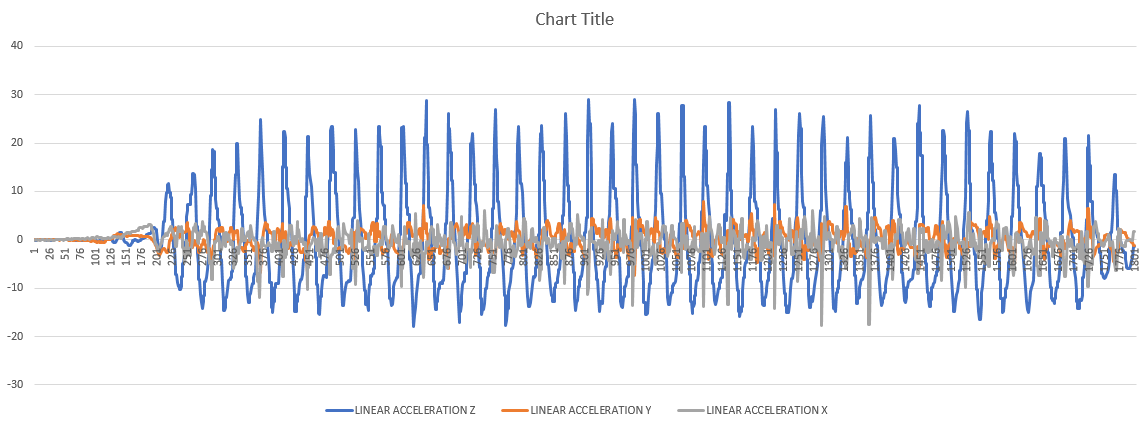
\includegraphics[width=\linewidth]{figures/accel.png}
\caption{}
\label{fig:accel}
\end{figure}
From this graph it it the rythmic motion of running is easy to see. a spike of close to 4g seen at the moment of impact and a maximum acceleration of around 1 g as the subject reaches maximum height.

\begin{figure}[!ht] 
\captionsetup{width=\linewidth, font=small}  
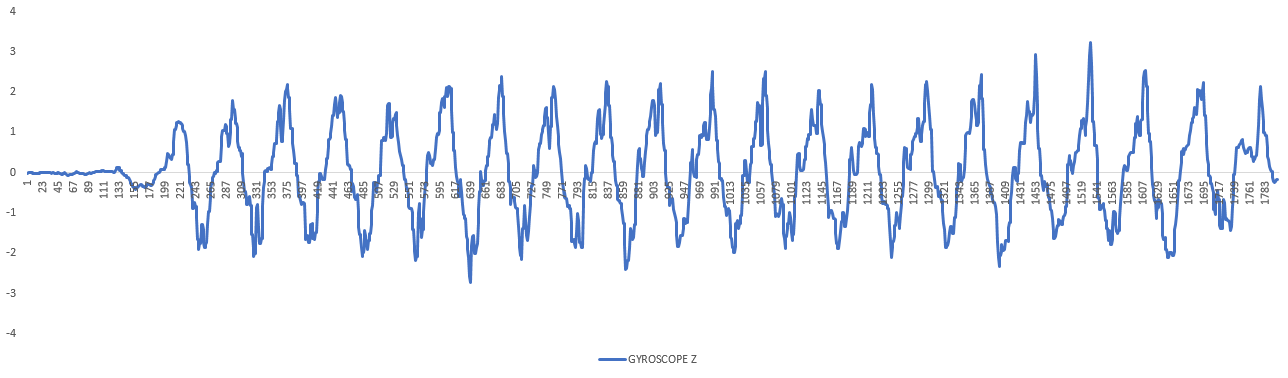
\includegraphics[width=\linewidth]{figures/gyroz.png}
\caption{}
\label{fig:gyroz}
\end{figure}

after image processing

\begin{figure}[!ht] 
\captionsetup{width=\linewidth, font=small}  
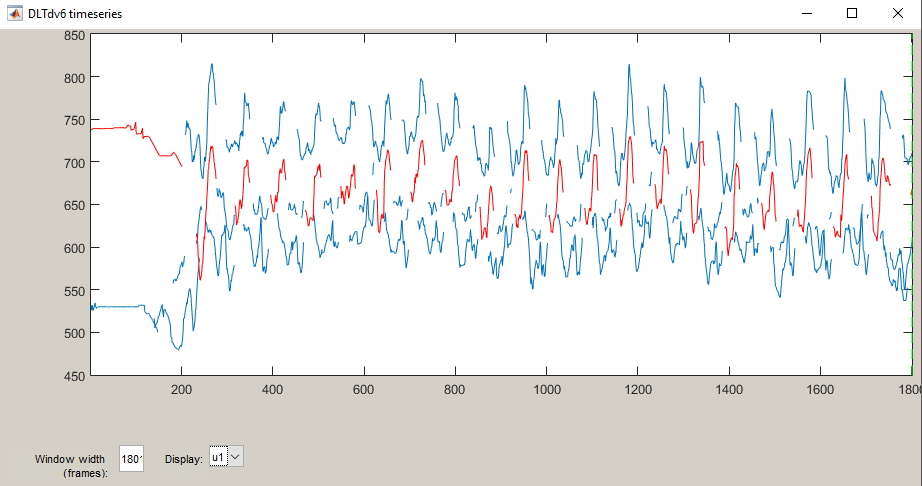
\includegraphics[width=\linewidth]{figures/ipdatapattern.png}
\caption{iamge processing things}
\label{fig:ipdatapattern}
\end{figure}



\subsection{EFK Results}



\section{Discussion}
subject borne cameras are have shown their viability. 












